% This is based on the LLNCS.DEM the demonstration file of
% the LaTeX macro package from Springer-Verlag
% for Lecture Notes in Computer Science,
% version 2.4 for LaTeX2e as of 16. April 2010
%
% See http://www.springer.com/computer/lncs/lncs+authors?SGWID=0-40209-0-0-0
% for the full guidelines.
%

\documentclass{llncs}

\usepackage[noend]{algpseudocode}
\usepackage{algorithm}
\usepackage{algorithmicx}

\usepackage{amsmath}
\usepackage{wrapfig}
\usepackage{amssymb}
\usepackage{tikz}
\usepackage{tikz-cd}
\usepackage[customcolors]{hf-tikz}
\usetikzlibrary{positioning,chains,fit,shapes,calc}
\usetikzlibrary{shapes.geometric, arrows}
\usetikzlibrary{automata}
\usepackage{tkz-graph}
\usepackage{tikz-cd}
\usepackage{varwidth}
\usepackage{qtree}
\usepackage{mathtools}
\usepackage{tabularx}
\usepackage{stmaryrd} %for \varoast (circle with asterisk)
\usepackage{subfig}
\usepackage[titletoc,title]{appendix}

\newlength\Colsep
\setlength\Colsep{10pt}

\usetikzlibrary{decorations.markings}

\newcommand{\e}{\emptyset}

\DeclareMathOperator{\Perm}{Perm}
\DeclareMathOperator{\Conj}{Conj}
\DeclareMathOperator{\SimultConj}{SimultConj}
\DeclareMathOperator{\len}{length}
\DeclareMathOperator{\ret}{ret}

\setcounter{tocdepth}{1}

\pagestyle{plain}

\title{Verifying Robustness of Programs Under Structural Perturbations}
\author{Jacob Bond and Clay Thomas}
\institute{Purdue University}

\begin{document}

\maketitle
% \tableofcontents

% \begin{abstract}
% \end{abstract}

\section{Introduction}

The question of robustness is fundamental to the subject of programming by
example (PBE).  Robustness of a program is the property that the program behaves
predictably on uncertain inputs \cite{chaudhuri12}.  In the PBE paradigm, there
is, by definition, an uncertainty regarding the intent of the user.  Therefore,
it is desirable that a program synthesizer behave predictably with regard to
this uncertainty.

Consider an attempt to specify the \(\max\) function by providing to a program
synthesizer the examples \((3, 5) \mapsto 5\), \((-7, 9) \mapsto 9\), and
\((-5, -8) \mapsto -8\).  In order to synthesize a simpler program, the
result will be the program \verb!P(a,b):=return b;!.  The issue that arises here
is that neither the program syntehsizer, nor the synthesized program, are
robust.

The program synthesizer is not robust, as transposing the inputs of each example
would result in the program \verb!P(a,b):=return a;!, while transposing just a
single input would result in the correct program \verb!P(a,b):=return a>b?a:b;!.

Additionally, the program which is synthesized is not robust as
\verb!P(a,b)!\(\not=\) \verb!P(b,a)!.  That is, the program does not behave
predictably under uncertainty in the order of the arguments.  If the program
which is synthesized is required to be robust with respect to uncertainty in the
order of the input, neither \verb!P(a,b):=return a;! nor \verb!P(a,b):=return b!
would be viable candidates, and the synthesizer would be forced to return
\verb!P(a,b):=return a>b?a:b;!.

Moreover, a synthesizer which returns robust programs will itself be more
robust.  Let \(\mathcal{I}_{1} = (I_{1}, O_{1})\) and \(\mathcal{I}_{2} =
(I_{2}, O_{2})\) be two input-output pairs for a program synthesizer which
differ by a small perturbation.  If the program \(\mathcal{P}_{1}\) returned by
the synthesizer on input \(\mathcal{I}_{1}\) is robust, then
\(\mathcal{P}_{1}(I_{2})\) will approximate \(O_{2}\) because \(I_{2}\)
approximates \(I_{1}\).  For this reason, \(\mathcal{P}_{2}\), the program
returned on input \(\mathcal{I}_{2}\), should only differ from
\(\mathcal{P}_{1}\) by a small amount.

Thus, the issue of robustness in PBE can be addressed by verifying robustness,
either of the synthesized programs or even of the synthesizer as a whole.
However, verification of robustness requires the ability to reason about
robustness.  Standard program verifiers are unable to verify robustness
properties as they are an example of a \(2\)-safety property, a property which
requires reasoning about two execution traces simultaneously.  Rephrasing the definition,
robustness is the property that given two inputs which are related by some form
of uncertainty, the outputs should be related in a predictable way.  As such,
verifying robustness requires reasoning about the relationship between two
execution traces.

\vspace{-0.1in}
\section{Related Work}

%  \subsection{Initial Approaches}
%    \noindent{\it\bf Relational Logics:}\space\space Benton \cite{benton} established a
%    Relational Hoare Logic in order to reason about relational properties,
%    properties which consider two, usually distinct, programs.  Barthe et al.
%    \cite{barthecrypto,bartheprivacy} extended Benton's Relational Hoare Logic to
%    probabalistic programs in order to reason about cryptographic protocols and
%    differential privacy.
%    \smallskip
%
%    \noindent{\it\bf Self-Composition:}\space\space Barthe et al.
%    \cite{barthecomposition} applied self-composition, sequential running of renamed
%    copies of the original program, to study secure information flow.  Terauchi \&
%    Aiken \cite{terauchi05} built on this work by applying a type-based approach to
%    complement self-composition.
%
%    \vspace{-0.1in}
  \subsection{Continuity and Lipschitz Robustness}
    \noindent{\it\bf Continuity:}\space\space Robustness in the setting of numerical perturbations
    is realized by the property of continuity.  Hamlet \cite{hamlet02} considered the
    concept of program continuity, but declared that automating verification of
    continuity for programs with loops was infeasible.  However, Chaudhuri et al.
    \cite{chaudhuri10} was able to establish a program logic which allowed such
    automatic verification of continuity.
    \smallskip

    \noindent{\it\bf Lipschitz Robustness:}\space\space 
    In many situations, the result of a program should be relatively
    stable with respect to uncertainty in the input.  That is, if the input is
    perturbed, the output should vary only slightly, relative to the input
    perturbation. This is exactly the concept of Lipschitz continuity (see Appendix A.1).

    Verifying the property of Lipschitz continuity is considered by Chaudhuri et al.
    \cite{chaudhuri11}.  The approach taken is to verify continuity of
    the program as a whole using \cite{chaudhuri11} and then verify that each control flow path of the
    program is piecewise Lipschitz continuous by showing that it is piecewise
    linear.  The continuity verification is performed using a program logic for
    reasoning about continuity \cite{chaudhuri10}.  In order to establish that each
    control flow path is piecewise linear, an abstract interpretation is applied in
    which an abstract state, referred to as a robustness matrix, is propagated to
    determine each rate of change \(\partial x_{i}^{out}/\partial x_{j}^{in}\).
    However, the approach used in
    \cite{chaudhuri10,chaudhuri11} is limited to numerical perturbations,
    and it is not clear how to adapt them to structural changes in the input.

    Additionally, Samanta et al. \cite{samanta13} and
    Henzinger et al. \cite{samanta14} investigate the use of Lipschitz continuity
    for proving robustness in the context of transducers.

  \subsection{$k$-Safety Properties}
    \noindent{\it\bf \(2\)-Safety Properties:}\space\space In \cite{terauchi05},
    Terauchi \& Aiken introduced the term \(2\)-safety property in the study of secure information flow.
    A general approach to verifying \(2\)-safety properties is the creation of a
    product program which is then provided as input to a standard program verifier
    \cite{bartheproduct}.  The product \(\mathcal{P}_{1} \varoast \mathcal{P}_{2}\)
    of two programs \(\mathcal{P}_{1}, \mathcal{P}_{2}\) is a program which is
    equivalent to simultaneously executing both \(\mathcal{P}_{1}\) and
    \(\mathcal{P}_{2}\).  Because a single program is created with distinct
    variables corresponding to each variable of \(\mathcal{P}_{1}\) and
    \(\mathcal{P}_{2}\), relational properties between \(\mathcal{P}_{1}\) and
    \(\mathcal{P}_{2}\) can be expressed as a standard verification property of the
    single program \(\mathcal{P}_{1} \varoast \mathcal{P}_{2}\).  As a result, a
    \(2\)-safety property about \(\mathcal{P}\), such as robustness, can be
    established by providing \(\mathcal{P} \varoast \mathcal{P}\) to any standard
    program verifier.

    In \cite{bartheanalysis}, Barthe et al.
    analyzes different notions of product programs, as well as various relational program logics and relationships between them.
    \smallskip

    \noindent{\it\bf \(k\)-Safety Properties:}\space\space Clarkson \& Schneider
    \cite{clarkson08} introduced \(k\)-safety properties as a generalization of 
    these ideas. Sousa \& Dillig \cite{sousa16} developed a program logic based on product programs
    to reason about \(k\)-safety properties.  Their approach is more efficient than
    using product programs as they avoid creation of an actual product program, while
    still being able to reason about properties of such a program.  Moreover, rather than
    considering a single product program, their approach considers the equivalence
    class of programs which are equivalent to the product program
    \(\mathcal{P}_{1} \varoast \dotsb \varoast \mathcal{P}_{k}\) and attempts to
    find an element of this equivalence class which is particularly easy
    to reason about.

    However, the result of these improvements is that their method is not compatible
    with a standard program verifier. Sousa \& Dillig developed
    an implementation of their algorithm, though it is limited to the verification
    of Java comparators.
    Discussion with the authors indicated that many structural invariants could
    be verified with this framework, but that the existing implementation is
    heavily specialized and would require new features in order to handle objects like
    arrays or trees.

\section{Example Robustness Properties}

  The uncertainty with respect to which a program is robust can take many
  different forms.  Some common perturbations include numerical perturbations
  \cite{samanta14,chaudhuri10,chaudhuri11} and permutations of arrays and matrices.
  As the case of continuous robustness is handled in \cite{chaudhuri10,chaudhuri11},
  the focus will be discrete perturbations.  In the context of discrete perturbations, it makes sense to consider perturbations of the input which leave the output invariant, as this situation is more common than in the case of continuous perturbations.

  \subsection{Integer Perturbations}

  A first example of uncertainty under a discrete perturbation is the presence
  of noise in a program operating on integer arrays.  However, because Lipschitz
  robustness with respect to \(\mathbb{R}\) implies Lipschitz robustness with
  respect to \(\mathbb{Z}\), this problem is a special case of the approach in
  \cite{chaudhuri10,chaudhuri11}.  As an example, sorting algorithms are
  \(1\)-Lipschitz robust by \cite{chaudhuri10,chaudhuri11}.
  If each element of the input array is perturbed by at most
  \(1\), then each element of the output array will be perturbed by at most \(1\).

  \vspace{-0.1in}
  \subsection{Permutations}

    %\begin{multline*}N = \len(a_{1}) \wedge \exists s. \Perm(s, N) \wedge \forall i. 0

    \subsubsection{Sorting}

      Sorting gives an example of a procedure which is robust with respect to permuting
      the input.  Even in the face of uncertainty regarding the order of the input
      array, the result of procedure will not be altered.  The \verb!max! function is
      a special case of this invariance of sorting algorithms under permutation, which
      is the root of the failures to synthesize the \verb!max!
      function in Section 1.

    \vspace{-0.1in}
    \subsubsection{Searching}

      Consider the function \verb!Find(a, x)! which returns the index of the element
      \verb!x! in the array \verb!a! or \(-1\) if \verb!x! is not an element of
      \verb!a!.  Let \(\sigma\) be a permutation and suppose that \verb!a[i]=x!.
      As discussed in Appendix A.2, we have
      \[
        \sigma\verb!a[!\sigma(\verb!i!)\verb!]! = \verb!a[i]! = \verb!x!,
      \] 
      so that \verb!Find(!\(\sigma\)\verb!a, x)=!\(\sigma(\)\verb!i!\()\).
%      Considering \(\sigma\) as a permutation on nonnegative integers, \(\sigma(-1) =
%      -1\) and \verb!Find(!\(\sigma\)\verb!a, x)=!\(\sigma(\)\verb!i!\()\) holds even
%      in the case that \verb!x! is not an element of \verb!a!.  
      Thus, \verb!Find! is
      robust in that perturbing the input array by a permutation \(\sigma\) perturbs
      the output of \verb!Find! by the same permutation.% \(\sigma\).

    \vspace{-0.1in}
    \subsubsection{Adjacency Matrices}

      The effect of permuting the rows and columns of an adjacency matrix by the same
      permutation is simply a relabelling of the vertices.  This leads to the following
      two robustness properties.  If the program computes a
      property of the graph, such as the existence of a Hamiltonian cycle, the program
      should be invariant under such a relabelling.  If the program computes a result
      which depends on the labelling, such as finding an explicit Hamiltonian cycle,
      the program should satisfy the that
      the output will be perturbed by the same permutation as the input.

\section{Invariance under permuting lists}
\label{permlists}

  As discussed above, many programs are invariant under the reordering of a list.
  Results from group theory  suggest a powerful 
  reduction from checking invariance of a list under all permutations
  to invariance under a set of just two permutations.
  Some background is discussed in Appendix A.2.
  In the languages discussed there, we want to verify that
  $\mathcal{P}(\sigma a) = \mathcal{P}(a)$ for every $\sigma\in S_n$.

  For any $n$, define
  \[
    \alpha = 
      \begin{tabular}{c@{\hspace{1em}}c@{\hspace{1em}}c@{\hspace{1em}}c@{\hspace{1em}}c@{\hspace{1em}}c}
      0 & 1 & 2 & \ldots & n-2 & n-1\\
      1 & 2 & 3 & \ldots & n-1 & 0
      \end{tabular}
    \qquad \qquad
    \beta = 
      \begin{tabular}{c@{\hspace{1em}}c@{\hspace{1em}}c@{\hspace{1em}}c@{\hspace{1em}}c@{\hspace{1em}}c}
      0 & 1 & 2 & 3 & \ldots & n-1\\
      1 & 0 & 2 & 3 & \ldots & n-1
      \end{tabular}
  \]

  \begin{lemma} \label{lem-generated}
    Every permutation is a composition of some sequence of $\alpha$ and $\beta$.
  \end{lemma}
  \begin{proof}
    This is a standard exercise in courses on group theory,
    where it is expressed by saying ``$\{\alpha,\beta\}$ generates 
    the group $S_n$''.
    See, for example, [Exercises 3-4, \S3.5, \cite{dummitfoote}].
  \end{proof}

  Thus, each $\sigma \in S_n$ is of the form $\sigma = $
  $\sigma = u_1 \circ u_2 \circ \ldots \circ u_m$ with
  $u_i \in \{\alpha,\beta\}$.
  So if we know that $P(\alpha s) = P(s)$ and $P(\beta s) = P(s)$,
  then 
  \[ P((u_1\circ u_2\circ \ldots u_m)s)
      = P((u_1 \circ \ldots \circ u_{m-1})s)
    = \ldots = P(u_1s) = P(s)
  \]


  \subsection{Application to programs}

    Let \(F\) and \(G\) be the formulas
    \begin{gather*}
        F: a_{1}[0] = a_{2}[1] \wedge a_{1}[1] = a_{2}[0] \wedge 
          \forall i.\big( 2 \leq i < \len(a_{1}) \rightarrow a_{1}[i] = a_{2}[i] \big) \\
          G:  a_{1}[\len(a_{1})-1] = a_{2}[0] \wedge \forall i. 0 \leq i < \len(a_{1})-1 \rightarrow a_{1}[i] = a_{2}[i+1]
    \end{gather*}
    $F$ expresses that $a_2 = \alpha a_1$ and $G$ expresses that 
    $a_2 = \beta a_1$.
    Thus, lemma~\ref{lem-generated} tells us that
    invariance of a program with respect to permuting its input
    can be expressed in the language of \cite{sousa16} as
    \[
      \|\len(a_{1}) = \len(a_{2}) \wedge (F \vee G)\| \ 
        \mathcal{P}(a) \  \|\ret_{1} = \ret_{2}\|.
    \]

  \subsection{Automata}
    In this subsection, we show that this reduction is especially powerful for
    analyzing deterministic finite automata.

    For a fixed $n$ and $\sigma \in S_n$, we can construct a finite state
    transducer $T$ such that $T(s) = \sigma s$ for $|s|=n$.  However, this does
    not provide any reasonable way of checking that a given finite state machine
    is invariant under any permutation of the input string.  Instead, we will
    construct finite state transducers $T_{\alpha}$ and $T_{\beta}$ such that
    for any $n$ and any string $s$ with $|s|=n$, we have $T_{\alpha}(s)=\alpha s$
    and $T_{\beta}(s) =\beta s$. Then, determining whether a FSM $M$ is
    invariant under permutation of its inputs is equivalent to determining
    whether
    \[
      L(M \circ T_\alpha) = L(M) = L(M \circ T_\beta)
    \]

    \begin{theorem}
      There is an algorithm for determining whether a deterministic finite state
      machine $M$ is invariant under permuting it input.
      The algorithm runs in time $O(n|\Sigma|^2\log(n|\Sigma|))$,
      where $n$ is the number of states of $M$.
    \end{theorem}

    As discussed, it suffices to construct $T_\alpha$ and $T_\beta$
    and check language equality.

    We first construct $T_\alpha$.
    For each symbol $a \in \Sigma$,
    $T_\alpha$ has a transition from its start
    state $s_0$ to $s_a$, while reading input $a$ and
    writing output $\epsilon$.
    For each $a\in \Sigma$ and each $b\in\Sigma$ with $b\ne \$$, there is a
    transition from $s_a$ to $s_a$, reading $b$
    and writing $b$.
    Then for each $a$, there is a transition from
    $s_a$ to $s_1$, reading $\$$ and writing $a\$$.

    We now construct $T_\beta$.
    For each symbol $a \in \Sigma$,
    $T_\beta$ has a transition from its start
    state $s_0$ to $s_a$, while reading input $a$ and
    writing output $\epsilon$.
    Each $s_a$ has a transition to $s_1$ while
    reading input $b$ (for any $b\in \Sigma$)
    and writing output $ba$.
    Then $s_1$ simply has transitions to $s_1$,
    reading any $a\in \Sigma$ and writing
    back $a$.

    The automata $T_\alpha$ and $T_\beta$ each have $O(|\Sigma|)$ states.
    Now, as discussed in Appendix A.2, the automata 
    $M \circ T_\alpha$ and $M \circ T_\beta$ have $O(n|\Sigma|)$ states.
    Determining language equality can then be done by minimizing the number of
    states of each of these FSMs, because minimal FSMs are unique \cite{hopcroft71}.
    This can be done, for example, by Hopcroft's algorithm \cite{hopcroft71},
    yielding a total runtime of $O(n|\Sigma|^2\log(n|\Sigma|))$.

    \begin{figure}[h]
      \centering
      \subfloat[][The automata $T_{\alpha}$]{
        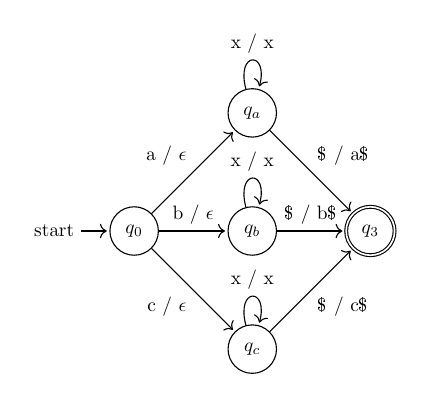
\begin{tikzpicture}[shorten >=1pt, node distance=1.5cm, on grid,
            auto, scale=0.8, every node/.style={scale=0.7}
        ] 
          \node[state,initial] (q_0)   {$q_0$}; 
          \node[state] (q_b) [right=of q_0] {$q_b$}; 
          \node[state] (q_a) [above=of q_b] {$q_a$}; 
          \node[state] (q_c) [below=of q_b] {$q_c$}; 
          \node[state, accepting] (q_1) [right=of q_b] {$q_3$};
          \path[->] 
          (q_0) edge node {a / $\epsilon$} (q_a)
                edge node {b / $\epsilon$} (q_b)
                edge node [below left] {c / $\epsilon$} (q_c)
          (q_a) edge node {\$ / a\$} (q_1)
                edge [loop above] node {x / x} (q_a)
          (q_b) edge node {\$ / b\$} (q_1)
                edge [loop above] node {x / x} (q_b)
          (q_c) edge node [below right] {\$ / c\$} (q_1)
                edge [loop above] node {x / x} (q_c)
                ;
        \end{tikzpicture}
      }
      \qquad
      \qquad
      \subfloat[][The automata $T_{\beta}$]{
        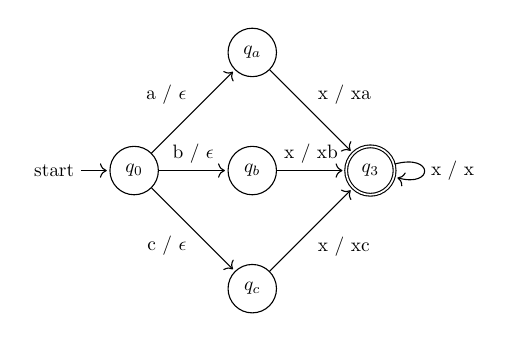
\begin{tikzpicture}[shorten >=1pt, node distance=1.5cm, on grid,
            auto, scale=0.8, every node/.style={scale=0.7}
        ] 
          \node[state,initial] (q_0)   {$q_0$}; 
          \node[state] (q_b) [right=of q_0] {$q_b$}; 
          \node[state] (q_a) [above=of q_b] {$q_a$}; 
          \node[state] (q_c) [below=of q_b] {$q_c$}; 
          \node[state, accepting] (q_1) [right=of q_b] {$q_3$};
          \path[->] 
          (q_0) edge node {a / $\epsilon$} (q_a)
                edge node {b / $\epsilon$} (q_b)
                edge node [below left] {c / $\epsilon$} (q_c)
          (q_a) edge node {x / xa} (q_1)
          (q_b) edge node {x / xb} (q_1)
          (q_c) edge node [below right] {x / xc} (q_1)
          (q_1) edge [loop right] node {x / x} (q_1)
                ;
        \end{tikzpicture}
      }
      \caption{Examples of our transducers when $\Sigma = \{a,b,c\}$}
    \end{figure}


    \vspace{-0.05in}
\section{Invariance under permuting binary search trees}
\vspace{-0.05in}

  In the previous section, we found a reduction
  from checking \emph{all} permutations of a list to checking a small set of
  permutations. It is natural to ask if there are other data types for which we
  can do this. Binary search trees are one such case, where just like lists,
  two permutations suffice to generate all equivalent binary search trees
  (i.e. trees representing equivalent ordered lists).

  We define binary search trees recursively as either being null,
  or having exactly two children who are binary search trees.
  Let \verb!list! be the function from a binary search trees to 
  its corresponding list, i.e. the function giving the in-order traversal of the
  tree's nodes.

  Define two (partial) operations $\rho$ and $\theta$ on binary search trees
  as in Figure~\ref{fig-rho-theta}.

  \begin{figure}[h]
    \centering

    \qroofx=2
    \qroofy=1
    \begin{tabular}{ccc}
     \Tree [.b [.a \qroof{LL}. \qroof{LR}. ] \qroof{R}. ]
        & \raisebox{-0.3in}{\ \ \ $\xmapsto{\ \ \rho\ \ }$ \!\!\!\!}
        & \Tree [.a \qroof{LL}. [.b \qroof{LR}. \qroof{R}. ]  ]
      \\
      \Tree [.c [.a \qroof{LL}. [.b \qroof{LRL}. \qroof{LRR}. ]] \qroof{R}. ]
        & \raisebox{-0.5in}{\ \ \ $\xmapsto{\ \ \theta\ \ }$ \!\!\!\!}
        & \Tree [.c [.b [.a \qroof{LL}. \qroof{LRL}. ] \qroof{LRR}. ] \qroof{R}. ]
    \end{tabular}
    \caption{The tree operations $\rho$ and $\theta$}
    \label{fig-rho-theta}
  \end{figure}

  One can verify that $\rho$ and $\theta$ preserve $\mathrm{list}(t)$
  by observing that the subtrees in the above diagrams remain in the same order
  before and after applying the transformations.
  We will show in the next theorem that $\rho$ and $\theta$ suffice
  to generate all transformations of one tree into any other tree with the same 
  underlying list.

  \begin{theorem}
    If a program $P$ on binary search trees is invariant under $\rho$
    and $\theta$, then whenever $\mathrm{list}(t_1) = \mathrm{list}(t_2)$,
    we have $P(t_1) = P(t_2)$.
  \end{theorem}
  \begin{proof}
    Let $t_1$ and $t_2$ satisfy $\mathrm{list}(t_1) = \mathrm{list}(t_2)$.
    Observe that if $P$ is invariant under $\rho$ and $\theta$,
    then $P$ is also invariant under $\rho^{-1}$ and $\theta^{-1}$.
    Thus, it suffices to show that $t_1$ and $t_2$ can both be transformed
    via $\rho$, $\theta$, $\rho^{-1}$, and $\theta^{-1}$ into another tree $t_3$,
    because then we can transform $t_1$ into $t_3$, then apply the inverse
    transformation of $t_2 \rightarrow t_3$.
    We proceed by providing an algorithm for transforming to a $t_3$
    in the following form, as demonstrated in
    figure~\ref{fig-tree-ops}\subref{fig-degenerate-list}:

    \begin{definition}
      A tree $t$ is in degenerate list form if either
      \begin{enumerate}
        \item $t$ is null, or
        \item $t$ has a null left child, and $t$'s right child is in degenerate
          list form.
      \end{enumerate}
    \end{definition}

    It is clear that if $t_1$ and $t_2$ are in degenerate list form, then
    $\mathrm{list}(t_1) = \mathrm{list}(t_2)$ if and only if $t_1 = t_2$.
    Thus, if we can show that $t_1$ and $t_2$ can both be transformed into
    degenerate list form, say $t_1'$ and $t_2'$, then we will have $t_1' = t_2'$
    and we will be done.

    Consider the following algorithm for adjusting a tree via $\rho$ and $\theta$,
    where invariants and assertions are written inside \{braces\}:

    \vspace{-0.2in}
    \begin{algorithm}
      \begin{algorithmic}[1]
        \Function{Listify}{$t$}
          \While{$t$ has a right child}
            \State apply $\rho^{-1}$ to $t$
          \EndWhile
          \State{\{$t$ has a null right child\}} \label{null-right}
          \While{$t$ has a left child}
            \Comment{\{$t$'s right child is in degenerate list form\}}
            \While{$t$'s left child has a right child}\label{inner-loop}
              \State apply $\theta$ to $t$
            \EndWhile
            \State{\{$t$'s left child has a null right child\}}
              \label{null-left-right}
            \State apply $\rho$ to $t$ \label{apply-rho}
          \EndWhile
          \State{\{$t$ is in degenerate list form\}} \label{postcond}
        \EndFunction
      \end{algorithmic}
    \end{algorithm} 
    \vspace{-0.1in}

    To verify that this algorithm terminates with $t$ in degenerate list form,
    we need only verify that each of the assertions hold and that the loop
    invariant is inductive.

    The invariant on line~\ref{null-right} follows from the negation of the
    condition of the loop before it.
    The loop invariant holds from line~\ref{null-right} simply because the null
    tree is in degenerate list form.
    The invariant on line~\ref{null-left-right} also follows from the negation of
    the condition of the loop before it.

    Next we show that the loop invariant is inductive.
    The inner loop on line~\ref{inner-loop} does not change $t$'s right child,
    so it remain in degenerate list form.
    Thus, when we apply $\rho$ to $t$, its left child has a null right child, and
    $t$'s right child is in degenerate list form.
    As shown in figure~\ref{fig-tree-ops}\subref{fig-apply-rho}, this leave $\rho(t)$'s right subtree
    in degenerate list form. 
    Thus, the invariant is inductive.

    Finally, we see that our conclusion on line~\ref{postcond} follows from the
    loop invariant and the negation of the condition, by the definition of
    degenerate list form.
    \begin{figure}
      \centering

      \vspace{-0.2in}
      \subfloat[][A tree in degenerate list form]{
        \label{fig-degenerate-list}
        \hspace{0.8in}
        \begin{tabular}{c}
          \Tree [.a $\e$ [.b $\e$ [.c $\e$ d ]]]
        \end{tabular}
        \hspace{0.8in}
      }
      \qquad
      \qquad
      \subfloat[][Applying $\rho$ to a tree as in line~\ref{apply-rho}]{
        \label{fig-apply-rho}
        \qroofx=2
        \qroofy=1
          \begin{tabular}{ccc}
            \Tree [.b [.a \qroof{LL}. $\e$ ] \qroof{R}. ]
            & \raisebox{-0.3in}{\ \ \ $\xmapsto{\ \ \rho\ \ }$ \ }
            & \Tree [.a \qroof{LL}. [.b $\e$ \qroof{R}. ]]
          \end{tabular}
      }
      \caption{}
      \label{fig-tree-ops}
    \end{figure}
%    \vspace{-0.4in}

  \end{proof}

  \section{Class invariance with respect to a function}

  All previous work on these topics share one downside: they require programmers
  to express their invariants in formal logic. 
  This could potentially be difficult,
  especially if the programmer is not formally trained.
  Here is one class of invariants that can be expressed through code:

  \begin{definition} We say that a program $P$ is class invariant with respect to a
    function $f$ if whenever $f(x)=f(y)$, we have $P(x)=P(y)$.
  \end{definition}

  For example, if a programmer defines a tree or heap data type with a function
  $\mathrm{list}$ mapping the data type to lists,
  then nearly every function written on this data type should be invariant with
  respect to the $\mathrm{list}$ function,
  as these data types are meant to represent the lists perfectly (while allowing
  for faster algorithms).

  We regard this problem as very difficult, because the function $f$ can be
  expressed with arbitrary code and thus encode more complicated properties than
  first order logic. One approach comes from the following observation:

  \begin{lemma} Let $P : S \to Z$ and $f : S \to T$.
    Then $P$ is $f$-class invariant if and only if
    there exists a program $\widetilde{P} : T\to Z$
    such that $P = \widetilde{P} \circ f$
  \end{lemma}
    \[
      \begin{tikzcd}
        S \arrow{rr}{P} \arrow{rd}{f} &   & Z \\
        & T \arrow[dashed]{ru}{\widetilde{P}} &   \\
      \end{tikzcd}
    \]
    \vspace{-0.3in}
  \begin{proof}
    If $P$ is $f$-class invariant, then the function
    \[ \widetilde{P}(t) = \begin{cases}
         P(s), & t = f(s) \text{ for some $s\in S$} \\
         z_0, & \text{otherwise}
       \end{cases}
    \]
    for any $z_0 \in Z$
    is well defined and clearly satisfies $P = \widetilde{P} \circ f$.

    Conversely, if $\widetilde{P}$ exists, then whenever $f(s)=f(s')$,
    we have $P(s) = \widetilde{P}(f(s)) = \widetilde{P}(f(s')) = P(s')$,
    so $P$ is $f$-class invariant.
  \end{proof}

  Now, the key observation is that $P$ and $f$ together give a full functional
  specification for $\widetilde{P}$.
  We want to either construct such a $\widetilde{P}$ in order to prove our
  property, or provide the programmer with a counterexample to the property in
  order to help them debug.
  Thus, a counterexample guided synthesis loop,
  similar to that present in \cite{solar06},
  seems like a natural candidate for this problem.

  \begin{figure}[h]
    \tikzstyle{process} = [rectangle, minimum width=3cm, minimum height=1cm,
      text centered, draw=black, fill=orange!30,
      text width=10em ]
    \tikzstyle{smallprocess} = [rectangle, minimum width=3cm, minimum height=1cm,
      text centered, draw=black, fill=orange!30,
      text width=6em ]
    \tikzstyle{io} = [rectangle, rounded corners,
      minimum width=3cm, minimum height=1cm,
      text centered, draw=black, fill=blue!30]
    \tikzstyle{arrow} = [thick,->,>=stealth]

    \begin{tikzpicture}[node distance=2cm, scale=0.8, every node/.style={scale=0.8}]
      \node (start) [io] {
        Input $P$ and $f$.
        Let $E = \{ \}$.
      };
      \node (synth) [process, below of=start, yshift=-0.5cm] {
        \textbf{Synthesize} a program $\widetilde{P} : S \to Z$
        given examples $\{ (f(t), P(t)) | t\in E \}$
      };
      \node (verify) [process, right of=synth, xshift=4cm] {
        \textbf{Verify} whether $\widetilde{P}\circ f$
        is equivalent to $P$
      };
      \node (yes) [io, above of=verify] {
        return YES
      };
      \node (check) [process, below of=verify, yshift=-1cm] {
        Check if there are any $t\in E$ such that
        $f(t)=f(t_0)$, yet $P(t) \ne P(t_0)$
      };
      \node (no) [io, below of=check, yshift=-0.5cm] {
        return NO
      };
      \node (add) [smallprocess, below of=synth, yshift=-1cm] {
        Add $t_0$ to the example set $E$
      };

      \draw [arrow] (start) -- (synth);
      \draw [arrow] (synth) -- (verify);
      \draw [arrow] (verify) --
        node[anchor=west, text width=6cm] {No, with \\ counterexample $t_0\in BSTs$}
        (check);
      \draw [arrow] (verify) --
        node[anchor=west, text width=6cm] {Yes, equivalent}
        (yes);
      \draw [arrow] (check) --
        node[anchor=north, text width=2cm, text centered] {No, $t$ does not exists}
        (add);
        \draw [arrow] (add) -- (synth);
      \draw [arrow] (check) --
        node[anchor=west, text width=6cm] {Yes, $t$ exists}
        (no);
    \end{tikzpicture}
    \caption{Decision procedure for verifying $f$-class invariance}
    \label{invarFuncLoop}
  \end{figure}

  It turns out this algorithm is sound, assuming a sound equivalence-of-programs
  verifier.
  If we assume a sound and complete synthesizer (meaning that there is
  always some set of examples that will result in a successful synthesis)
  and verifier, the algorithm is relatively complete.
  However, we need to assume one additional condition on the
  equivalence-of-programs verifier.
  Namely, we suppose there is some total order on the elements in $T$,
  and that if $\widetilde{P}\circ f$ is not equivalent to $P$,
  the verifier outputs the smallest counterexample with respect to this
  ordering.

  \begin{theorem}
    The algorithm in figure~\ref{invarFuncLoop} is sound and relatively complete,
    relative to a perfect synthesizer and a perfect equivalence-of-programs
    verifier.
  \end{theorem}
  \begin{proof}

    If $\widetilde{P}$ exists, then a perfect synthesizer will eventually
    synthesize $\widetilde{P}$ given some set of examples, say $E$.
    Because the verifier gives back counterexamples in a fixed order,
    a superset of $E$ will eventually be fed into the synthesizer,
    resulting in $\widetilde{P}$.
    Then the idealized verifier will output ``YES''.

    If no $\widetilde{P}$ exists, then some pair $t, t_0$ exist
    such that $f(t)=f(t_0)$ yet $P(t)\ne P(t_0)$.
    Because the verifier outputs counterexamples in some order,
    $t$ and $t_0$ will eventually be found, and the algorithm will output ``YES''.
  \end{proof}

\section{Conclusion}

While PBE suffers from some amount of uncertainty in a user's intent, synthesizing
a robust program can mitigate some of this uncertainty.  To this end, we explored
various approaches related to verifying the robustness of a program, as well as
different robustness properties a program can possess.  We discovered a reduction
for the problem of verifying permutation invariance in arrays and binary search trees,
and proposed a counterexample guided synthesis approach to verifying more general
invariance properties.

Directions for future research include an implementing methods for verifying robustness
in order to determine their usability as part of a synthesis procedure.  Specifically,
we would like to implement the product program approach of \cite{bartheproduct}, the
Cartesian Hoare Logic method of \cite{sousa16}, and our approach of synthesizing a
\(\widetilde{P}\) program to verify invariance.

\appendix

\vspace{-0.1in}
\section{Appendix: Background}

  \subsection{Lipschitz Robustness}

    Lipschitz continuity of a mathematical function \(f\) is the property that there
    exists a real number \(K \in \mathbb{R}^{+}\) so that for all \(x_{1}, x_{2}\),
    \(d\big(f(x_{1}), f(x_{2})\big) \leq K\,d(x_{1}, x_{2})\).  Similarly, a program
    \(\mathcal{P}\) is robust at a state \(\sigma\)  with respect to the input
    variable \(x_{in}\) and output variable \(x_{out}\) if for all \(\varepsilon \in
    \mathbb{R}^{+}\), whenever \(\sigma'\) satisfies
    \(d\big(\sigma(x_{in}), \sigma'(x_{in})\big) < \varepsilon\) and
    for all \(y \not= x_{in}\), \(\sigma(y) = \sigma'(y)\),
    we have \(d\big(\mathcal{P}(\sigma)(x_{out}), \mathcal{P}(\sigma')(x_{out})\big) < K\varepsilon\),
    where \(K\) is a real-valued function of the size of \(x_{in}\)
    \cite{chaudhuri11}.

    \vspace{-0.1in}
  \subsection{Permutations}
  \label{perms}

    A permutation is a bijection from a set \(\Omega\) to itself \cite{dummitfoote}.
    When \(\Omega\) is a finite set, a permutation can be specified using two-line
    notation by placing the elements of \(\Omega\) on one line, and their images
    under \(\sigma\) beneath them:

    % increase the intercolumn spacing
    \begin{center}
    \begin{tabular*}{0.5\textwidth}{c@{\extracolsep{\fill}}c}
    \(\sigma\):
    \begin{tabular}{c@{\hspace{1em}}c@{\hspace{1em}}c@{\hspace{1em}}c@{\hspace{1em}}c@{\hspace{1em}}c}
    0 & 1 & 2 & 3 & 4 & 5\\
    5 & 2 & 3 & 1 & 4 & 0
    \end{tabular}
    &
    \(\tau\):
    \begin{tabular}{c@{\hspace{1em}}c@{\hspace{1em}}c}
    a & b & c\\
    a & c & b
    \end{tabular}
    \end{tabular*}
    \end{center}

    Similar to two-line notation, a permutation on \(\{0, \dotsc, N-1\}\) can be
    encoded in an array \(a\) of length \(N\) by placing the image of \(i\) in
    \(a[i]\).  The example \(\sigma\) above is encoded in an array as \(\sigma = [5,
    2, 3, 1, 4, 0]\), so that \(\sigma(i) = \sigma[i]\).
    The inverse of a permutation is defined as for general inverse functions,
    so $\sigma^{-1}$ sends $\sigma(i)$ to $i$.

  \paragraph{Action on an Array:}

    Given a permutation \(\sigma\), \(\sigma\) can {\it act} on an array or list \(a\)
    by permuting the entries of $a$.
    For example, let \(a = [37, 25, 19, 49, 81, 21]\) and \(\sigma\) be as above.  
    Then \(\sigma(3) = \sigma[3] = 1\) and applying \(\sigma\) to \(a\) results in the
    element of \(a\) at index \(3\), \(49\), being moved to index \(1\) in \(\sigma
    a\).  That is, \(\sigma a[1] = 49\) and \(a[3] = \sigma a[1] = \sigma
    a[\sigma[3]]\).  More generally,
    \begin{equation}
    \sigma a[\sigma[i]] = a[i] \qquad 
      \Longleftrightarrow \qquad \sigma a[i] = a[\sigma^{-1}[i]]
    \label{action}
    \end{equation}

    \vspace{-0.1in}
  \subsection{Automata}
    We consider two classes of automata: finite state machines (FSM) and finite
    state transducers (FST). All automata we consider are deterministic. Given an
    automata $A$, we denote by $A(s)$ the output of $A$ on input $s$. If $A$ is a
    FSM, we represent ``accept'' by $1$ and ``reject'' by $0$. Otherwise, $A$ is a
    finite state transducer (FST), and $A(s)$ is a string. For a FSM $A$, let $L(A)$
    denote the set of strings accepted by $A$. (We do not define the language of a
    FST).

    Recall that for any FSMs $A$ and $B$, the problem of determining whether $L(A) =
    L(B)$ is decidable. We can compose a FST $T$ and a FSM $A$, denoted $A \circ T$,
    to get another FSM such that $(A\circ T)(s) = A(T(s))$.
    Furthermore, $A\circ T$ can be constructed with $|S_A||S_T|$ states,
    where $S_A$ and $S_T$ are the states of $A$ and $T$.
    % For example, $A\circ T$ can be constructed with set of
    % states $S_A \times S_T$, where $S_A$ and $S_T$ are the states of $A$ and $T$,
    % and with transition function
    % \[ \delta_{A\after T}((a,t), c) = (\delta_A( , \delta_T(t,c))
    % \]
    We will assume that all input strings are terminated by a special end-of-input character \$.

%
% ---- Bibliography ----
%
\bibliographystyle{splncs}
\bibliography{robustness}


\end{document}

%\titlerunning{Verifying Alegebraic Proper}
% abbreviated title (for running head)
% also used for the TOC unless \toctitle is used
%\authorrunning{Ivar Ekeland et al.} % abbreviated author list (for running head)
%%%% list of authors for the TOC (use if author list has to be modified)
%\tocauthor{Ivar Ekeland, Roger Temam, Jeffrey Dean, David Grove,
%Craig Chambers, Kim B. Bruce, and Elisa Bertino}
%\email{I.Ekeland@princeton.edu},\\ WWW home page:
%\texttt{http://users/\homedir iekeland/web/welcome.html}
%\and
%Universit\'{e} de Paris-Sud,
%Laboratoire d'Analyse Num\'{e}rique, B\^{a}timent 425,\\
%F-91405 Orsay Cedex, France}
